\PassOptionsToPackage{usenames, dvipsnames}{xcolor}
\documentclass[tikz, 10pt]{standalone}
\usepackage{fontspec}
  \defaultfontfeatures{Ligatures={NoCommon, NoDiscretionary, NoHistoric, NoRequired, NoContextual}, Mapping=tex-text}
  \setmainfont{Times New Roman}
\usepackage{xcolor}
\usepackage{graphicx}
\usepackage{relsize}
\usepackage{tikz, tikz-qtree}
	\usetikzlibrary{shapes, arrows, backgrounds, fit, positioning}

\begin{document}
  \begin{tikzpicture}[node distance=4em, anchor=west, align=flush center, FLOW/.style={->, very thick}, LABEL/.style={draw, fill=yellow!80, inner sep=.75em}, scale = 2, transform shape]
  	\node{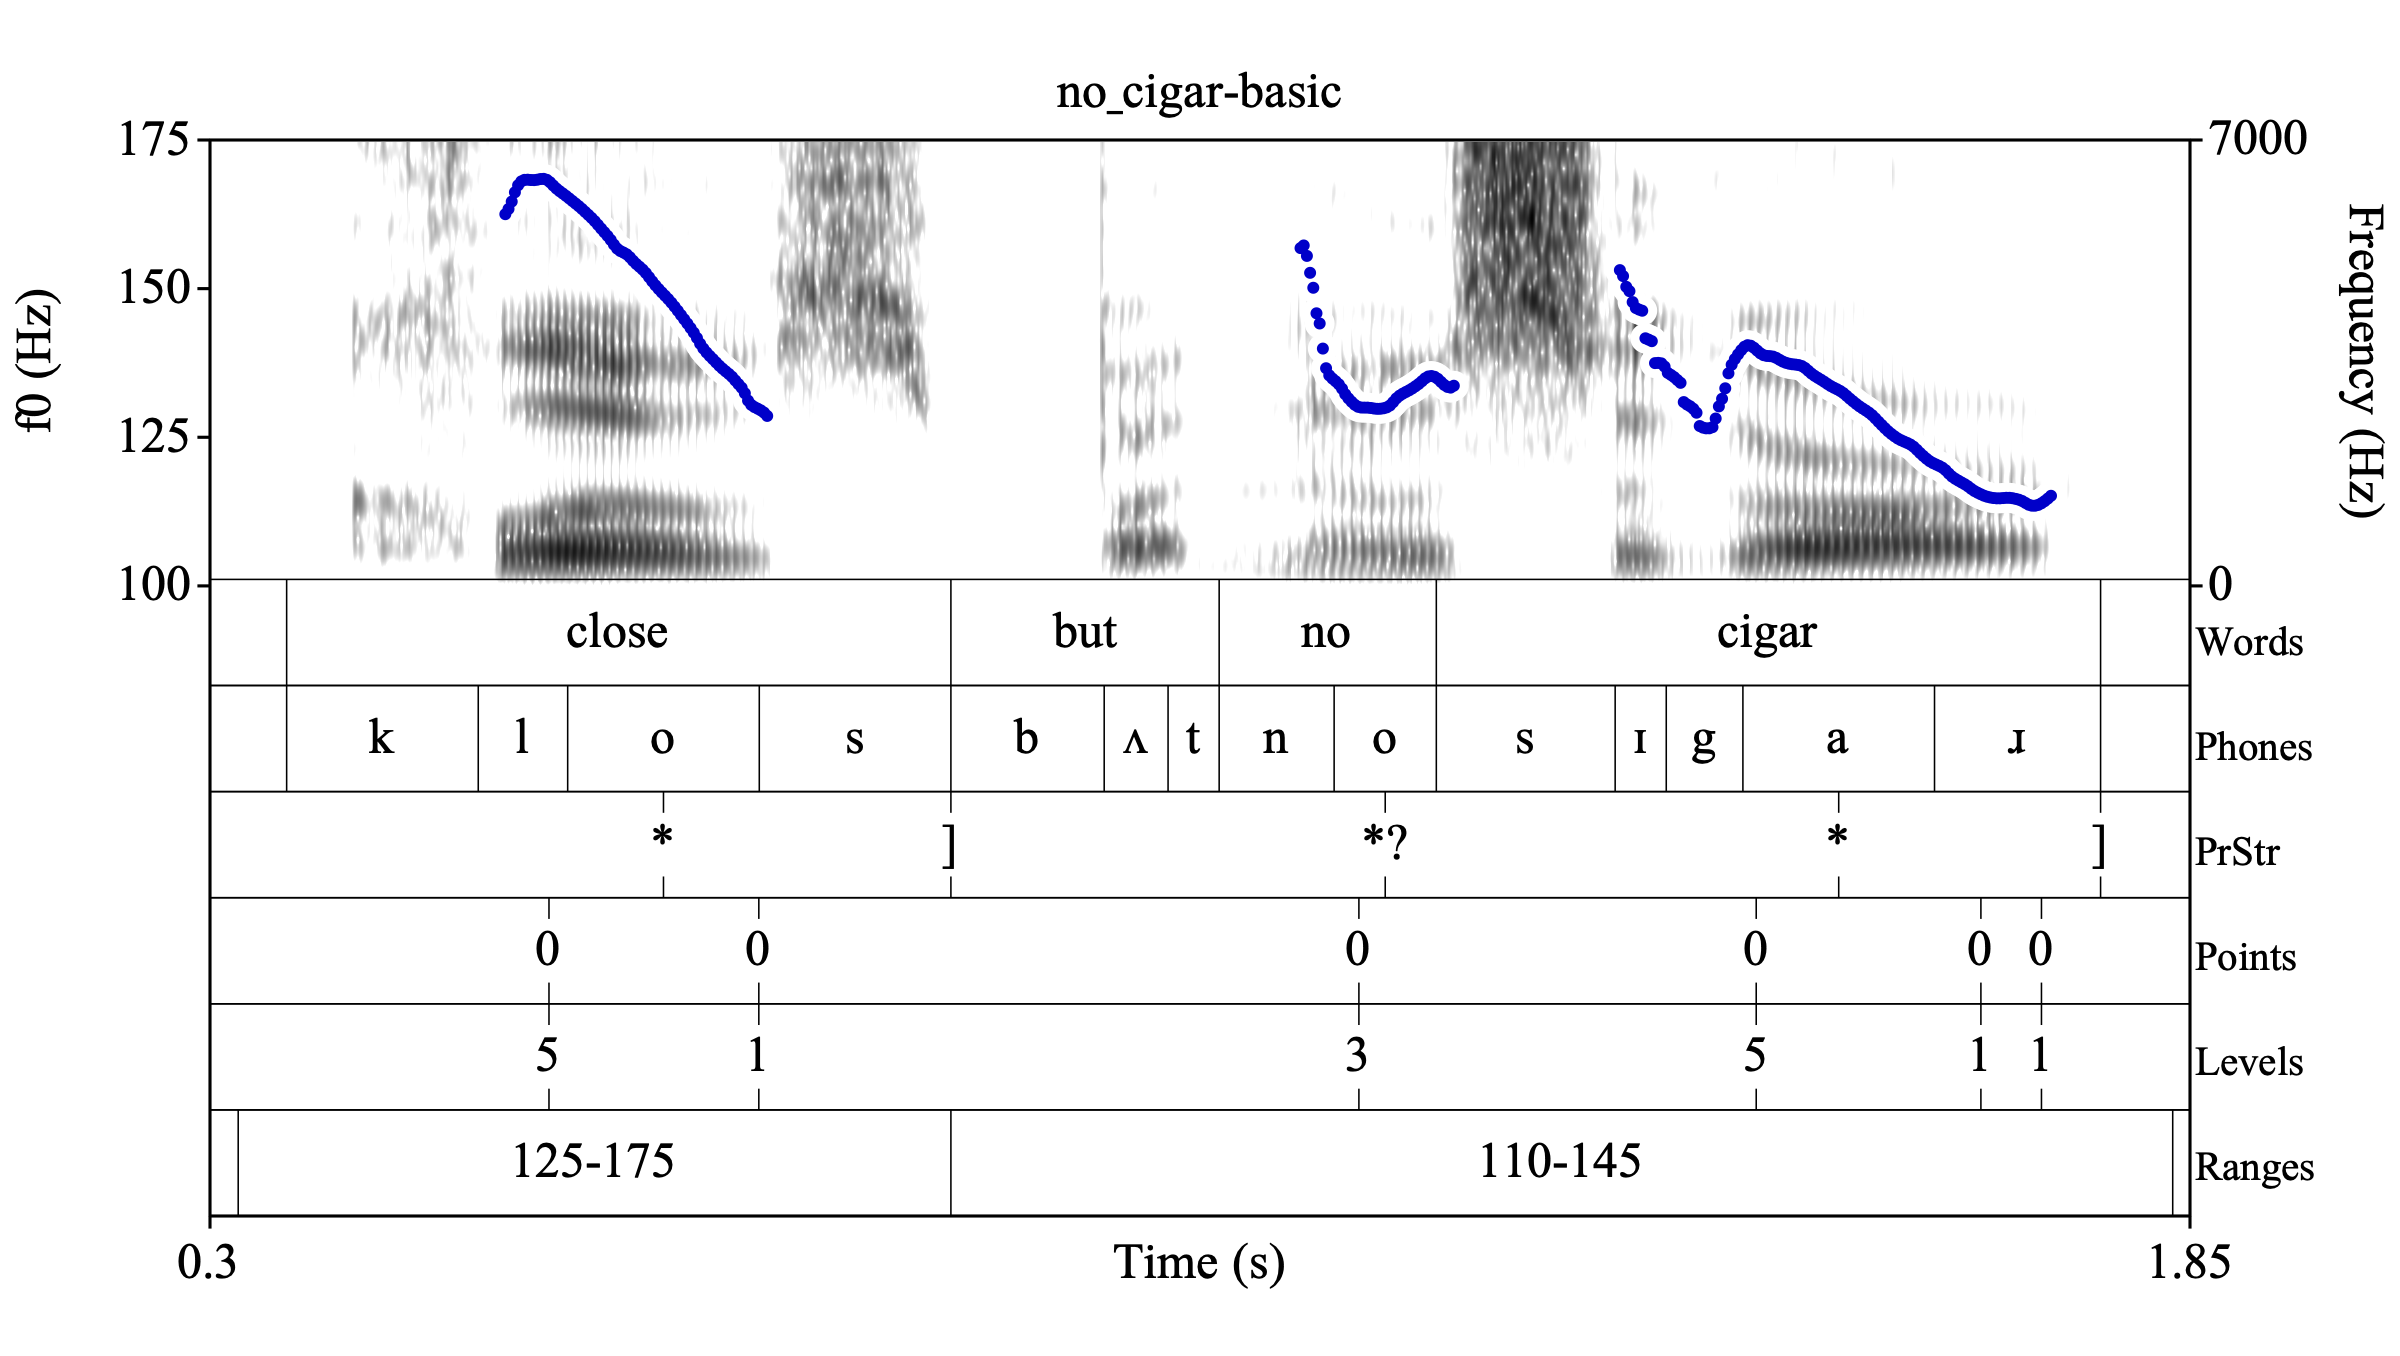
\includegraphics[width=25em]{Levels-no_cigar-basic.png}};
    \draw [black, fill=violet!30, opacity=.5] (1, 0.88) rectangle (3.6, 1.096);
    \draw [black, fill=blue!30, opacity=.5] (1, 1.096) rectangle (3.6, 1.312);
    \draw [black, fill=green!30, opacity=.5] (1, 1.312) rectangle (3.6, 1.528);
    \draw [black, fill=yellow!30, opacity=.5] (1, 1.528) rectangle (3.6, 1.744);
    \draw [black, fill=red!30, opacity=.5] (1, 1.744) rectangle (3.6, 1.96);
	\draw[red, opacity=.35] (2.13, -1.2) -- (2.13, 1.95);
	\draw[red, opacity=.35] (2.9, -1.2) -- (2.9, 1.95);
%
    \draw [black, fill=violet!30, opacity=.5] (3.6, 0.552) rectangle (8, 0.704);
    \draw [black, fill=blue!30, opacity=.5] (3.6, 0.704) rectangle (8, 0.856);
    \draw [black, fill=green!30, opacity=.5] (3.6, 0.856) rectangle (8, 1.008);
    \draw [black, fill=yellow!30, opacity=.5] (3.6, 1.008) rectangle (8, 1.16);
    \draw [black, fill=red!30, opacity=.5] (3.6, 1.16) rectangle (8, 1.312);
	\draw[red, opacity=.35] (5.1, -1.2) -- (5.1, 1.95);
	\draw[red, opacity=.35] (6.55, -1.2) -- (6.55, 1.95);
	\draw[red, opacity=.35] (7.37, -1.2) -- (7.37, 1.95);
	\draw[red, opacity=.35] (7.59, -1.2) -- (7.59, 1.95);
%	\draw[step=.5, black] (2, 0) grid (8, -2);
  \end{tikzpicture}
\end{document}